\documentclass[border=2pt]{standalone}
\usepackage[dvipsnames,svgnames,x11names]{xcolor}
\usepackage{tikz}
\usetikzlibrary{calc,arrows.meta,positioning,fit,shapes.geometric}

\tikzset{
  funfig node/.style={
    draw,
    rounded corners=2pt,
    minimum height=8mm,
    inner xsep=7pt,
    inner ysep=4pt,
    align=center,
  },
  funfig arrow/.style={
    -{Stealth[length=5pt,width=4pt]},
    line width=0.65pt,
  },
}

\begin{document}
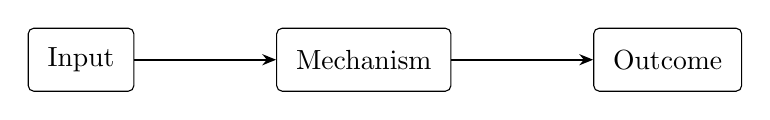
\begin{tikzpicture}[node distance=12mm and 18mm]
  \node[funfig node] (a) {Input};
  \node[funfig node,right=of a] (b) {Mechanism};
  \node[funfig node,right=of b] (c) {Outcome};

  \draw[funfig arrow] (a) -- (b);
  \draw[funfig arrow] (b) -- (c);
\end{tikzpicture}
\end{document}

